
\documentclass[10pt,a4paper]{article}
\usepackage[latin1]{inputenc}
\usepackage{color}
\usepackage{amsmath}
\usepackage{amsfonts}
\usepackage{amssymb}
\usepackage{graphicx}
\usepackage{listings}
\usepackage{color}
\definecolor{codegreen}{rgb}{0,0.6,0}
\definecolor{codegray}{rgb}{0.5,0.5,0.5}
\definecolor{codepurple}{rgb}{0.58,0,0.82}
\definecolor{backcolour}{rgb}{0.95,0.95,0.92}

\lstdefinestyle{mystyle}{
	backgroundcolor=\color{backcolour},   
	commentstyle=\color{codegreen},
	keywordstyle=\color{magenta},
	numberstyle=\tiny\color{codegray},
	stringstyle=\color{codepurple},
	basicstyle=\footnotesize,
	breakatwhitespace=false,         
	breaklines=true,                 
	captionpos=b,                    
	keepspaces=true,                 
	numbers=left,                    
	numbersep=5pt,                  
	showspaces=false,                
	showstringspaces=false,
	showtabs=false,                  
	tabsize=2
}
\lstset{style=mystyle}
\lstset{language=Java}
\usepackage[height=24.0cm]{geometry}
\author{Alex Foglia}
\title{Neural Networks and Statistical Models: A Java Implementation}
\begin{document}
	\maketitle
	\tableofcontents
	\newpage
	\section{Introduction}
	An Artificial Neural Network is a \emph{computational model} composed of a set of simpler and conceptually atomic sub-models called neurons, which goal is to simulate a biological brain, in particular the ability of this to learn. From a statistical point of view, Artificial Neural Networks (from here on, NN) are a wide class of nonlinear regression models, data reduction models, and \emph{non-linear} dynamical systems.\\*
	Neurons consist in interconnected computing elements (i.e. a neuron may compute a linear combination of some inputs) and they are often organized into \emph{layers}. For these reasons, it is convenient to graphically represent a NN through a directed graph, keeping in mind that represent a NN model means to represent a model that nothing has to do with \emph{Bayesian Networks}, always represented through a directed (acyclic) graph.\\*
	The alleged "intelligence" of a NN is a matter of dispute, since networks, like many statistical methods, are capable of processing vast amounts of data and making predictions, but this does not make them "intelligent" in the usual sense of the word. What engineers and computer scientists call "learning" is just what it is called "estimation" in the statistical jargon.\\*
	Most of the NN models are similar or identical to statistical techniques such as generalized linear models, polynomial regression, principal components and cluster analysis, etc, but there are also a few NN models that have no precise statistical equivalent but may be useful for data analysis.\\*
	Although many NN models are similar or identical to well-known statistical models, the terminology in the NN literature is quite different from that in statistics. Here it follows a brief table which explain such a difference.
	\\*
	\\*
	\begin{tabular}{|c|c|}
		\hline 
		\textbf{Statistical Jargon} & \textbf{NN Jargon} \\ 
		\hline 
		Variables & Features \\ 
		\hline 
		Independent Variable & Inputs \\ 
		\hline 
		Predicted Values & Outputs \\ 
		\hline 
		Dependent Variables & Targets \\ 
		\hline 
		Residual & Errors \\ 
		\hline 
		Estimation & Training, Learning \\ 
		\hline 
		Estimation Criterion & Error Function \\ 
		\hline 
		Observations & Patterns \\ 
		\hline 
		Parameter Estimates & Synaptic Weights \\ 
		\hline 
		Interactions & Higher-Order neurons \\ 
		\hline 
		Transformations & Functional Links \\ 
		\hline 
		Regression & Supervised Learning \\ 
		\hline 
		Data reduction & Unsupervised Learning \\ 
		\hline 
		Cluster Analysis & Competitive Learning \\ 
		\hline 
		Interpolation and Extrapolation & Generalization \\ 
		\hline 
	\end{tabular} \\*\\*
	Terms like \emph{sample} and \emph{population} does not have NN equivalents, but data are often divided into a \emph{training set} and \emph{test set} for cross-validation.
	\section{NN and Linear Regression Model}
	Linear regression models are simple statistical models used to predict the expected value of a \emph{dependent variable} $\textbf{Y}$ given a set of \emph{observed variables} $\textbf{X}$. The model is the following:
	$$
	\textbf{Y}_i = \beta_0 + \beta_1 \textbf{X}_i + \varepsilon_i
	$$
	Where $i$ variates between $1$ to $N$ where $N$ is the number of observations, $\textbf{Y}_i$ is the dependent variable, $\textbf{X}_i$ is the independent variable, $\beta_0 + \beta_1 \textbf{X}_i$ is the regression line and $\varepsilon_i$ is the statistical error. Parameters $\beta_0$ and $\beta_1$ are called respectively the intercept and the angular coefficient of the regression line, and they must be estimated in order to have a reliable prediction of the $\textbf{Y}$. To perform this task, it is often used the \emph{ordinary least square} method. $S$ is defined as:
	$$
	S(\beta_0,\beta_1) = \sum_{i=1}^N (y_i - \beta_0 - \beta_1 \textbf{X}_i)^2
	$$
	$S$ is a function from $\mathbb{R}^2 \rightarrow \mathbb{R}$ and parameters $\beta_0,\beta_1$ are estimated  as the arguments of $S$ on which the function evaluates to its minimum.\\*
	Consider the following NN:\\*
	\begin{figure}[h!]
		\centering
		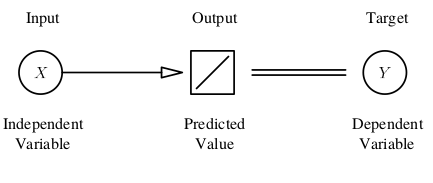
\includegraphics[scale=2.5]{img/linreg}
	\end{figure}\\*
	Boxes represent values computed as a function of one or more arguments, the symbol inside the box indicate the type of the function (in this case, it is a linear combination of the input).\\*
	Arrows indicate that the source of the arrow is an argument of the function computed at the destination of the arrow, and usually each arrow has a corresponding \emph{weight} (parameter in statistical jargon) to be estimated.\\*
	Two long parallel lines indicate that the values at each end are to be fitted by the ordinary least square method, or some other estimation criterion.\\*
	Such a NN represents the Linear Regression Model in the NN Jargon.
	\section{Logistic Regression: Perceptrons}
	A perceptron is a very small NN, composed by more than one neuron, and it usually computes a linear combination of the inputs.
	A perceptron has $n>0$ output. Each output has a specific \emph{weight} $\beta_i$. The \emph{weights} are the parameters to be estimated. In order to estimate $\beta_i$ parameters, it is used a specific \emph{activation function} which usually maps any real input to a bounded range. Bounded activation functions are called \emph{squashing functions}, for instance the logistic function:
	$$
	\texttt{act}(x) = \dfrac{1}{1+e^{-x}}
	$$
	Maps any real argument to the range $(0,1)$:
	$$
	\lim_{x\rightarrow +\infty} \dfrac{1}{1+e^{-x}} = 	\lim_{x\rightarrow +\infty} \dfrac{1}{1+\dfrac{1}{e^x}} = \dfrac{1}{1+0} = 1
	$$
	$$
	\lim_{x\rightarrow -\infty} \dfrac{1}{1+e^{-x}} = 	\lim_{x\rightarrow +\infty} \dfrac{1}{1+{e^x}} = \dfrac{1}{\infty} = 0
	$$
	The estimation is usually performed by the \emph{maximum likelihood} method, but another method, very used in NN context, is the \emph{gradient descendant}.\\*
	Suppose it exists a set of data that called training set. This is a set of pairs of  \texttt{input - expected output} and the aim is to minimize
	$$
	\sum \sum r_j^2
	$$
	Where the $r_j$ is the difference between the expected output and the predicted value.\\*
	The \emph{logisitc regression model} is a \emph{non-linear} regression model used when the dependent variable is dichotomic.\\*
	The model formulae is the following:
	$$
	\mathbb{E}(\textbf{Y}|\textbf{X}) = \dfrac{e^{\beta_0 + \beta_1x_1+\dots+\beta_n x_n}}{1 +e^{\beta_0 + \beta_1x_1+\dots+\beta_n x_n} }
	$$
	The following perceptron with a logistic activation function is a logistic regression model:
		\begin{figure}[h!]
		\centering
		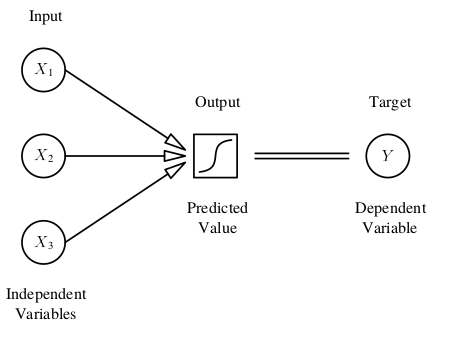
\includegraphics[scale=1.7]{img/logreg}
	\end{figure}\newpage
	\section{Nonlinear Regression: Multilayer Perceptrons}
	In the introduction section, it exposed that neurons are often organized into \emph{layers}. NN seen before are simple perceptrons composed of two layers: the input layer and the output layer. If it is introduced another \emph{hidden} layer between input and output, you obtain a multi-layer perceptron (MLP).\\*
	If the model includes estimated weights between the inputs and the hidden layer, and the hidden layer uses nonlinear activation functions such as the logistic function, the model becomes nonlinear.\\*
		\begin{figure}[h!]
		\centering
		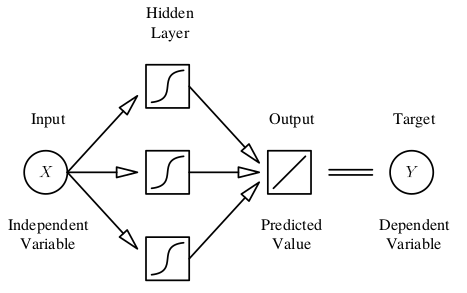
\includegraphics[scale=2.5]{img/nonlinreg}
	\end{figure}\\*
	This is a simple MLP implementing a non linear regression model:
	$$
	\textbf{Y} = f(\textbf{X}) + \textbf{b}
	$$
	MLP are general-purpose, flexible, nonlinear models that can approximate
	virtually any function to any desired degree of accuracy. MLP are called \emph{universal approximators} and they can be used when you have little knowledge about the relationship between the independent and dependent variables.
	\section{Java Implementation}
	Start from the linear regression model:
	$$
	\textbf{Y}_i = \beta_0 + \beta_1 \textbf{X}_i + \varepsilon_i
	$$
	\begin{figure}[h!]
		\centering
		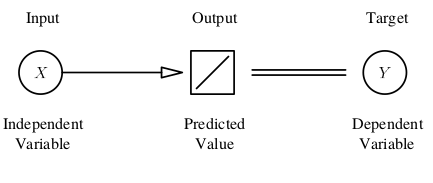
\includegraphics[scale=2]{img/linreg}
	\end{figure}\\*
	Suppose it is $\varepsilon_i = 0$ . Consider the following class:
	\begin{lstlisting}[language=Java]
public class Neuron {
private double b0,b1;
	
public double predict(double x) {
	return b0 + b1*x;
}
public static void main(String[] args) {
	Neuron y = new Neuron();
	System.out.println(y.predict(7));
}
}
	\end{lstlisting}
	It is clear that the output provided by the execution of this code it is \texttt{0.0}, and it is due to the fact that the $\beta_0,\beta_1$ parameters are not yet estimated. It is known that $\beta_0,\beta_i$ are estimated as the minima of the function
	$$
	S(\beta_0,\beta_1) = \sum_{i=1}^N (y_i - \beta_0 - \beta_1 x_i)^2
	$$
	As it is known in the mathematical analysis theory, it is possible to find the minima setting the partial derivatives equal to zero:
	$$
	\frac{\vartheta S}{\vartheta \beta_0} = -2 \sum_{i=1}^N (y_i - \beta_0 - \beta_1x_i) = 0,\;\;\;\;
	\frac{\vartheta S}{\vartheta \beta_1} = -2 \sum_{i=1}^N (y_i - \beta_0 - \beta_1 x_i) x_i = 0
	$$
	From which the following solutions are derived:
	$$
	\beta_1 = \frac{\sigma(x,y)}{\sigma^2(x)},\;\;\;\;
	\beta_0 = \overline y - \beta_1 \overline x
	$$
	Where $ x_i$ is the $i-th$ observation for which it is known a-priori the dependant variable value $y_i$;\\* $\sigma(x,y)$ is the covariance between variables $\textbf{X},\textbf{Y}$;\\* $\sigma^2(x)$ is the observed variance of the variable $\textbf{X}$;\\* $\overline x, \overline y$ are respectively the observed mean of the variable $\textbf{X}$ and the observed mean of the variable $\textbf{Y}$.\\*
	It is needed to extend the code adding the following piece of code:
	\begin{lstlisting}[language = Java]
public void estimateParameters(double[] xi, double[] yi) {
	b1 = var(xi,yi) / var(xi,xi);
	b0 = mean(yi) - b1*mean(xi);
}
private double mean(double[] v) {
	double m = 0;
	for(int i=0; i<v.length;i++) {
		m+=v[i];
	}
	return m/v.length;
}
private double var(double[] x, double[] y) {
	double var = 0;
	double mx = mean(x);
	double my = mean(y);
	for(int i=0; i<x.length;i++) {
		var+= (x[i]-mx)*(y[i]-my);
	}
	return var/x.length;
}
\end{lstlisting}
Suppose it exists a sample \textbf{X} for which it is known that all the values of the dependent variable \textbf{Y} are on the bisector of the second quadrant of the Cartesian plane:
$$
\textbf{X} = \{X_i\} = \{1,2,3,4,5\}
$$
$$
\textbf{Y} = \{Y_i\} = \{1,2,3,4,5\}
$$
\begin{lstlisting}[language = Java]
Neuron y = new Neuron();
y.estimateParameters(new double[]{1,2,3,4,5}, new double[]{1,2,3,4,5});
System.out.println(y.predict(7));
System.out.println("Y=" + y.b0 + "+" + y.b1+"X");
\end{lstlisting}
As it is expected, even if in the \emph{training set} does not appear the expected output for value $7$, our linear regression model is able to predict the output for such a value:
\begin{lstlisting}
7.0
\end{lstlisting}
In fact the regression line is exactly the requested identity function:
\begin{lstlisting}
Y = 0.0 + 1.0X
\end{lstlisting}
Consider now the logistic regression perceptron model:\\*
	\begin{figure}[h!]
	\centering
	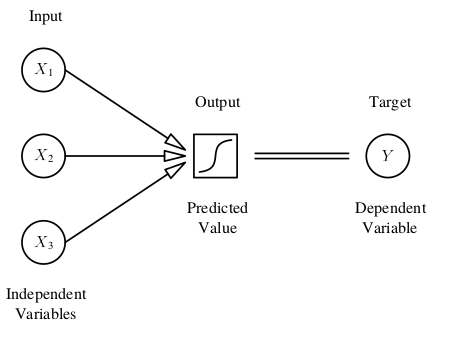
\includegraphics[scale=1.7]{img/logreg}
\end{figure}\\*
The code must be modified in order to implement a logistic regression model:
\begin{lstlisting}[language=Java]
public class Neuron {
	private double[] weights;
	
	public Neuron(int n_inputs) {
		weights = new double[n_inputs];
	}
	
	private double logistic(double x) {
		return 1 / (1 + Math.exp(-x));
	}
	
	public double predict(double[] inputs) {
		double sum = 0;
		for (int i = 0; i < inputs.length; i++) {
			sum += weights[i] * inputs[i];
		}
		return logistic(sum);
	}
}
\end{lstlisting}
Now there is an array of weights to be approximated, and the prediction is performed by applying the logistic function to the linear combination of the given inputs. Since weights are all zero by default, every invocation on the \texttt{predict()} method evaulates to \texttt{0.5} because
$$
\frac{1}{1+e^{0}} = \frac{1}{2} = 0.5
$$
Now the job is to modify the \texttt{estimateParameter()} method seen before in order to estimate weights using the gradient descent method:
\begin{lstlisting}[language=Java]
public void estimateParameters(double[][] xi, double[] yi) {
	double[] gradient = new double[weights.length];
		for (int i = 0; i < xi.length; i++) {
			for (int j = 0; j < xi[0].length; j++) {
				gradient[j] += (double) xi[i][j] *
				 (yi[i] - predict(xi[i]));
			}
		}
	for (int j = 0; j < weights.length; j++)
		weights[j] += gradient[j];
}
\end{lstlisting}
Note that the logistic function has a "friendly" derivative that permit us to compute its gradient in such an easy way.\\*
Consider this piece of python code:
\begin{lstlisting}[language=Python]
import math
b0 = 1
b1 = 2
squash = lambda x: math.exp(-(b0*x[0]+b1*x[1]))/(1+math.exp(-(b0*x[0]+b1*x[1])))
print squash([1,0])
print squash([0,1])
print squash([0,0])
print squash([1,1])
\end{lstlisting}
Executing it, it is possible to generate data from the logistic function:
$$
f(\textbf x) = \frac{e^{-x_1-2x_2}}{1+e^{-x_1-2x_2}},
$$
Obtaining:
$$
f(1,0) \;\approx\;0.2689414213699951, f(0,1) \approx 0.11920292202211755, f(0,0) = 0.5, f(1,1) \approx 0.04742587317756679
$$
It is possible now to train this simple network with such data:
\begin{lstlisting}[language=Java]
Neuron n = new Neuron(2);
double[][] in = {{1,0},{0,1},{0,0},{1,1}};
double[] out = {0.2689414213699951,0.11920292202211755,0.5,0.04742587317756679};
for(int i=0; i<10000;i++)
	n.estimateParameters(in, out);
System.out.println(Arrays.toString(n.weights));
\end{lstlisting}
Obtaining the following coefficients:
\begin{lstlisting}
[-1.0000000000000004, -1.9999999999999993]
\end{lstlisting}
Which are approximately the $\beta_0,\beta_1$ used to generate data but with the sign changed, in fact, in the Java program, it is used the following logistic function:
\begin{lstlisting}[language = Java]
private double logistic(double x) {
	return 1 / (1 + Math.exp(-x));
}
\end{lstlisting}
Which is:
$$
\frac{1}{1+e^{-x}}
$$
But in the python code, it is used:
$$
\frac{e^{-x}}{1+e^{-x}}
$$
For which it is:
$$
\frac{e^{-x}}{1+e^{-x}} = \frac{1}{1 + e^x}
$$
A simple try:
\begin{figure}[h]
	\centering
	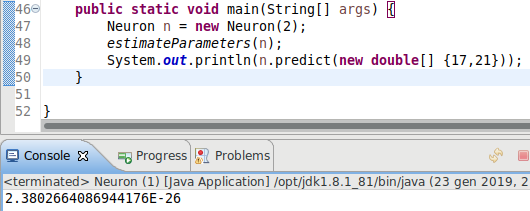
\includegraphics[scale=2]{img/logregpred}
	\label{fig:logregpred}
\end{figure}
\begin{figure}[h]
	\centering
	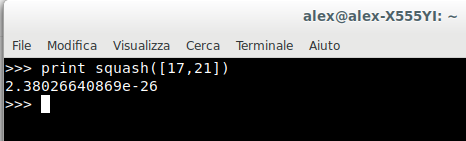
\includegraphics[width=0.7\linewidth]{img/logregpredpython}
	\label{fig:logregpredpy}
\end{figure}\newpage \noindent
Consider the following \emph{truth table}:
\begin{center}
\begin{tabular}{|c|c|c|}
	\hline 
	$x_1$ & $x_2$ & $x_1$ $\oplus$ $x_2$ \\ 
	\hline 
	0 & 0 & 0 \\ 
	\hline 
	0 & 1 & 1 \\ 
	\hline 
	1 & 0 & 1 \\ 
	\hline 
	1 & 1 & 0 \\ 
	\hline 
\end{tabular}\\*
\end{center} 
This is known as the logical operator \textit{xor}. A Neural Network is capable to learn the \textit{xor} computation of two logical variables.\\*
Consider the following NN Model:\\*
\begin{figure}[h]
	\centering
	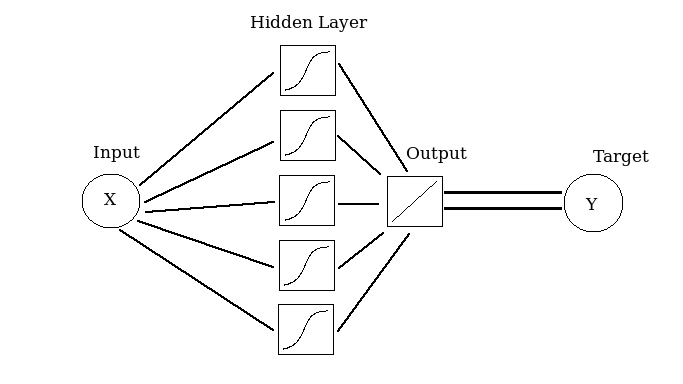
\includegraphics[width=0.7\linewidth]{img/mymodel}
	\label{fig:mymodel}
\end{figure}\\*
This is a MLP, or \emph{universal approximator}. The aim is to modify the provided code in order to implement such a MLP which is able to learn to compute the \emph{xor}.\\*
Start from the Neuron class\footnote{The information hiding principle has been completely ignored, in order to simplify the code}:
\begin{lstlisting}[language=Java]
public class Neuron {
	public double[] weights;
	public double[] inputs;
	public double output;
	public Neuron(int n_inputs) {
		weights = new double[n_inputs];
	}
	private double logistic(double x) {
		return 1/(1+Math.exp(-x));
	}
	public double predict(double[] inputs) {
		this.inputs = inputs;
		double sum = 0;
		for(int i=0; i<inputs.length;i++) {
			sum += inputs[i] * weights[i];
		}
		this.output = logistic(sum);
	return output;
	}
}
\end{lstlisting}
The main modification is that the \texttt{estimateParameters()} method will be moved in another class. Now a Neuron does also keep track of the provided inputs, this will be useful when it will be implemented the \emph{back-propagation algorithm}, an algorithm which estimate weights aiming to minimize the error between the predicted output and the desired output using the \emph{descent gradient} principle.\\*
Since MLPs have more than one layer, it is needed to define, from a programming point of view, what a layer is.\\*It is just a collection of Neurons:
\begin{lstlisting}[language=Java]
public class NeuronLayer {
	public Neuron[] neurons;
	public NeuronLayer(int n, int inputsPerNeuron) {
		this.neurons = new Neuron[n];
		for (int i = 0; i < n; i++) {
			this.neurons[i] = (new Neuron(inputsPerNeuron));
		}
	}
	
	public double[] feedForward(double[] inputs) {
		double[] outputs = new double[neurons.length];
		for (int i = 0; i < neurons.length; i++) {
			outputs[i] = (neurons[i].predict(inputs));
		}
		return outputs;
	}
	
	public double[] getOutputs() {
		double[] outputs = new double[neurons.length];
		for (int i = 0; i < neurons.length; i++) {
			outputs[i] = neurons[i].output;
		}
		return outputs;
	}
}
\end{lstlisting}
In this class it is defined the number of neurons the layer is composed of, the inputs that each neuron will handle (equivalently, the length of the vector of weights to estimate for each neuron) and two methods: the \texttt{feedForward()} which is a generalization of the \texttt{predict()} method defined for each neuron, and it returns a collection of prediction computed by each neuron; and the \texttt{getOutputs()} which simply collects each neuron's output without providing them of any input.\\* The scope here it is clear, we have implemented the MLP's hidden layer with a variable amount of hidden neurons:
\begin{figure}[h!]
	\centering
	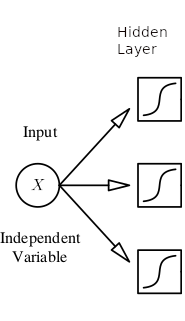
\includegraphics[scale=1.5]{img/hiddenlayer}
	\label{fig:hiddenlayer}
\end{figure}\newpage\noindent
Putting layers together means to construct a MLP Neural Network.
\begin{lstlisting}
public class NeuralNetwork {
	private int n_in,n_hid,n_out;
	private NeuronLayer hidden,output;
	public NeuralNetwork(int inputNeurons, int hiddenNeurons, int numberOfOutputs) {
		n_in = inputNeurons;
		n_hid = hiddenNeurons;
		n_out = numberOfOutputs;
		hidden = new NeuronLayer(n_hid, n_in);
		output = new NeuronLayer(n_out, n_hid);
	}
}
\end{lstlisting}
First of all, the MLP must initialize hidden and output layers neurons weights. The most recomended way is to perform this task using random values:
\begin{lstlisting}
public void initInputToHidden() {
	for (int i = 0; i < n_hid; i++) {
		for (int j = 0; j < n_in; j++) {
			hidden.neurons[i].weights[j] = Math.random();
		}
	}
}
public void initHiddenToOut() {
	for (int i = 0; i < n_out; i++) {
		for (int j = 0; j < n_hid; j++) {
			output.neurons[i].weights[j] = Math.random();
		}
	}
}
\end{lstlisting}
The MLP must be capable of performing prediction:
\begin{lstlisting}
public double[] feedForward(double[] inputs) {
	double[] hidden_outputs = hidden.feedForward(inputs);
	return output.feedForward(hidden_outputs);
}
\end{lstlisting}
Last, the MLP must be capable of being trained in order to estimate neurons weights:
\begin{lstlisting}
	public void train(double[] training_in, double[] training_out) {
	feedForward(training_in);
	double[] deltaWrtOut = new double[n_out];
	for (int i = 0; i < n_out; i++) {
		double target_output = training_out[i];
		double actual_output = output.neurons[i].output;
		double deltaWrtInput = -(target_output - actual_output) * actual_output * (1 - actual_output);
		deltaWrtOut[i] = deltaWrtInput;
	}
	double[] deltaWrtHid = new double[n_hid];
	for(int i=0; i<n_hid;i++) {
		double deltaWrtHiddenOut = 0;
		for(int j=0; j<n_out;j++) {
			deltaWrtHiddenOut+=deltaWrtOut[j] * output.neurons[j].weights[i];
		}
		double actual_output = hidden.neurons[i].output;
		double deltaWrtIn = actual_output * (1 - actual_output);
		deltaWrtHid[i] = deltaWrtHiddenOut * deltaWrtIn;
	}
	for (int i = 0; i < n_out; i++) {
		for (int j = 0; j < n_hid; j++) {
			double act_input = output.neurons[i].inputs[j];
			double deltaWrtWeight = deltaWrtOut[i] * act_input;
			output.neurons[i].weights[j] -= deltaWrtWeight;
		}
	}
	for (int i = 0; i < n_hid; i++) {
		for (int j = 0; j < n_in; j++) {
			double act_input = hidden.neurons[i].inputs[j];
			double deltaWrtWeight = deltaWrtHid[i] * act_input;
			hidden.neurons[i].weights[j] -= deltaWrtWeight;
		} } }
\end{lstlisting}
The logic of the method shown above is the logic of the \emph{back-propagation algorithm}. Another method is added in order to compute the total network error with respect to a training set:
\begin{lstlisting}
public double totalError(double[][][] training_sets) {
	double err = 0;
	for (int i = 0; i < training_sets.length; i++) {
		double[] t_in = training_sets[i][0];
		double[] t_out = training_sets[i][1];
		double[] act_out = feedForward(t_in);
		for (int j = 0; j < act_out.length; j++) {
			double target_output = t_out[j];
			double actual_output = output.neurons[j].output;
			double squareError = 0.5 * Math.pow(target_output - actual_output, 2);
			err += squareError;
		}
	}
	return err;
}
\end{lstlisting}
\subsection{MLP Training and Utilization}
Now the model is ready to being trained and utilized. Start from constructing the model shown at the top of this section. It has 2 inputs, 5 hidden neurons, 1 output:
\begin{lstlisting}
NeuralNetwork nn = new NeuralNetwork(2, 5, 1);
\end{lstlisting}
Define the training sets as defined in the \emph{xor} table of truth:
\begin{lstlisting}
double[][][] training_sets = {
{{0, 0}, {0}},
{{0, 1}, {1}},
{{1, 0}, {1}},
{{1, 1}, {0}}
};
\end{lstlisting}
Train the network:
\begin{lstlisting}
System.out.println("Error before training: "+nn.totalError(training_sets));
for (int i = 0; i < 20000; i++) {
	int randIndex = (int) (Math.random() * training_sets.length);
	double[] t_in = training_sets[randIndex][0];
	double[] t_out = training_sets[randIndex][1];
	nn.train(t_in, t_out);
}
System.out.println("Error after training: "+nn.totalError(training_sets));
\end{lstlisting}
And this is the output:
\begin{lstlisting}
Error before training: 0.7825167086789118
Error after training: 0.0019131802708672071
\end{lstlisting}
In the next page it follows a \texttt{main()} example.\\*
What it is implemented is a MLP which performs a \emph{xor} approximation using the statistical model \emph{non-linear regression}. The name \emph{universal approximator} has a powerful meaning. If you try to train the MLP with other datasets which arise from considering other functions than the \emph{xor}, such as the \emph{and}, \emph{nand}, etc, the MLP will approximate them with the same degree of accuracy.
\newpage
\begin{figure}
	\centering
	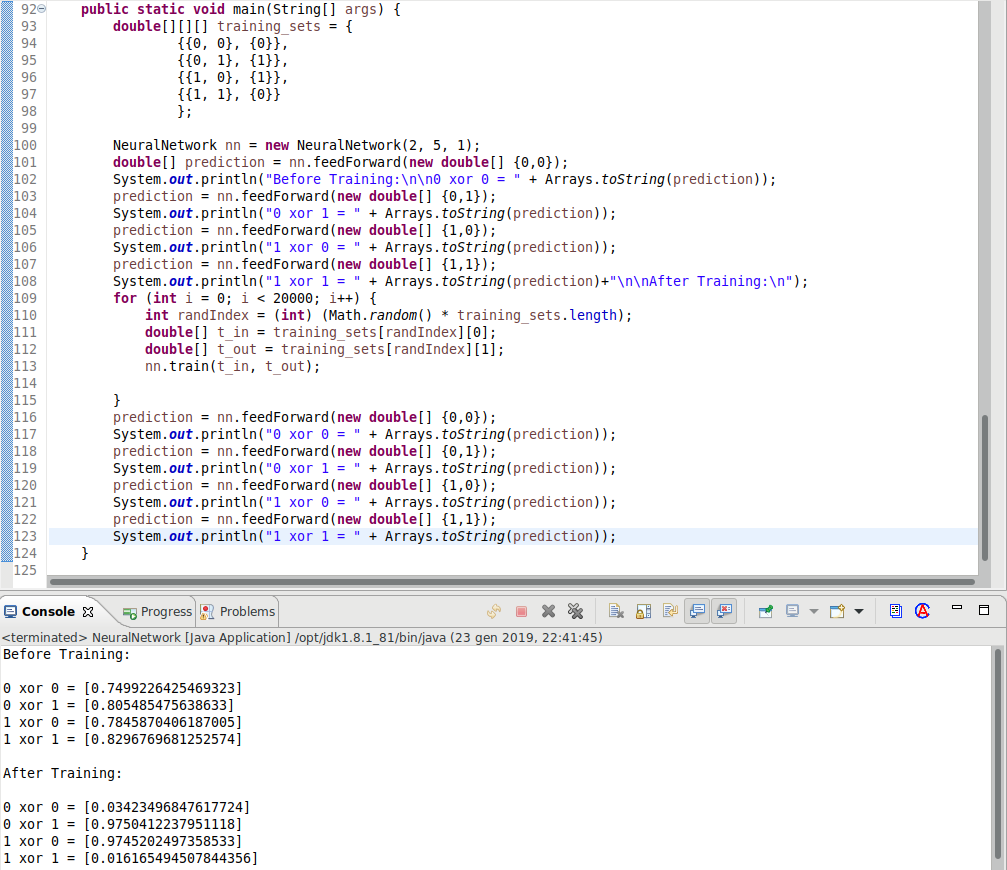
\includegraphics[scale=1.91]{img/nn}
	\label{fig:nn}
\end{figure}
\section{Conclusions}
In this study, based on the paper "Neural Networks and Statistical Model" by Warren S. Sarle, I illustrated the similarities between models of artificial neural networks and some known statistical regression models. Artificial neural networks are nothing more than a technical implementation of these theoretical models of estimation. The purpose of a regression model is to infer a function that is as close as possible to the real function that generated a certain set of data, always assuming that this function exists. Therefore, what is called "intelligence" of a Neural Network, is the degree of accuracy with which a certain regression model can approximate a distribution from which the data is assumed to be observed. My opinion is that the assumption underlying these models is very heavy, and we are still far away from a true reproduction of human intelligence. Moreover, when any artificial intelligence system is used, the questions we have to ask are:
\begin{itemize}
	\item Does a precise distribution for the data we have observed really exist?
	\item How was the sample formed?
\end{itemize}
These questions impose some important ethical consideration, since artificial intelligence systems are often used to profile human beings, as for example in the USA when the COMPAS software has been used by the Florida Supreme Court, to decide whether, after an interview to the suspect, it had to be kept in custody, and what the ransom was supposed to be.\\* Last, starting from the simple linear regression model, I implemented step by step a small Neural Network able to compute the xor of two Boolean variables, in Java language.
\end{document} 